\documentclass[12pt,a4paper]{report}

\usepackage[T1]{fontenc}
\usepackage[utf8]{inputenc}
\usepackage[french]{babel}
\usepackage{lmodern}
\usepackage[a4paper,margin=2.5cm]{geometry}
\usepackage{setspace}
\usepackage{graphicx}
\usepackage{float}
\usepackage{array}
\usepackage[table]{xcolor}
\usepackage{colortbl}
\usepackage{titlesec}
\usepackage{fancyhdr}
\usepackage[hidelinks]{hyperref}
\usepackage{tocloft}

\definecolor{headerblue}{HTML}{B4C6E7}

\graphicspath{{./images/}}
\setstretch{1.2}
\setcounter{secnumdepth}{3}
\setcounter{tocdepth}{3}

\pagestyle{fancy}
\fancyhf{}
\renewcommand{\headrulewidth}{0.8pt}
\fancyhead[L]{\itshape\leftmark}
\fancyfoot[C]{\thepage}

\titleformat{\chapter}[display]
  {\normalfont\bfseries\Huge}
  {Chapitre \Roman{chapter}}
  {0.8ex}
  {\Huge}

\titlespacing*{\chapter}{0pt}{-10pt}{24pt}

\makeatletter
\renewcommand{\chaptermark}[1]{%
  \markboth{Chapitre \thechapter.\ #1}{}%
}
\makeatother

\begin{document}

\begin{titlepage}
    \centering
    \vspace*{1.5cm}

    {\Large Republique Tunisienne\par}
    \vspace{0.3cm}
    {\large Ministere de l'Enseignement Superieur et de la Recherche Scientifique\par}
    \vspace{0.3cm}
    {\large Rapport de Projet de Fin d'Etudes\par}
    \vspace{2cm}

    {\Huge\bfseries HireCue\par}
    \vspace{0.4cm}
    {\LARGE Plateforme de recrutement intelligente basee sur l'IA\par}
    \vspace{2cm}

    \begin{tabular}{>{\bfseries}p{5cm}p{8cm}}
        Organisme d'accueil : & Teligencia Labs \\
        Nature du document : & Rapport PFE niveau ingenieur \\
        Theme : & Intelligence artificielle appliquee au recrutement \\
    \end{tabular}

    \vfill

    {\large Annee universitaire 2025--2026\par}
\end{titlepage}

\thispagestyle{empty}
\pagenumbering{gobble}
\chapter*{D\'edicace}

\thispagestyle{empty}
\vspace*{2cm}
Ce travail est d\'edi\'e d'abord aux parents et \`a M.~Taher Zayani, pour leurs efforts constants, leurs sacrifices, leur affection inconditionnelle et leur pr\'esence silencieuse, qui ont accompagn\'e chaque \'etape du parcours.

\vspace{0.8cm}

Leur confiance, leur patience et leur soutien ont constitu\'e une aide pr\'ecieuse tout au long des ann\'ees d'\'etude.

\vspace{0.8cm}

Il est \'egalement d\'edi\'e aux fr\`eres, Fares et Seif, pour leur pr\'esence, leurs encouragements et l'\'equilibre qu'ils ont su apporter dans les moments les plus difficiles.

\vspace{0.8cm}

Une pens\'ee sinc\`ere est aussi adress\'ee aux amis, dont l'\'ecoute, la bienveillance et le soutien moral ont rendu ce parcours plus apais\'e et plus enrichissant.

\vspace{0.8cm}

Que cette r\'ealisation soit l'expression d'une profonde reconnaissance envers toutes les personnes qui, d'une mani\`ere ou d'une autre, ont contribu\'e \`a la r\'ealisation de ce projet.

\chapter*{Remerciements}

La r\'ealisation de ce projet de fin d'\'etudes s'est appuy\'ee sur l'accompagnement et le soutien de plusieurs personnes auxquelles une sinc\`ere gratitude est adress\'ee.

Des remerciements particuliers sont d'abord adress\'es \`a Monsieur \textbf{Badis Messaoudi}, encadrant au sein de l'entreprise d'accueil, pour la qualit\'e de son suivi, la pertinence de ses orientations et la disponibilit\'e accord\'ee tout au long du stage. Son accompagnement a permis d'aborder le projet \textit{HireCue} dans un cadre professionnel exigeant, avec un niveau d'attention constant port\'e \`a la coh\'erence technique et \`a la valeur metier des \'evolutions r\'ealis\'ees.

Une reconnaissance particuli\`ere est \'egalement adress\'ee \`a Monsieur \textbf{Chedy Bouslema}, encadrant acad\'emique, pour ses conseils, ses remarques constructives et son appui m\'ethodologique. Ses orientations ont contribu\'e \`a mieux structurer ce travail et \`a maintenir une lecture acad\'emique coh\'erente des choix techniques et fonctionnels pr\'esent\'es dans le rapport.

Des remerciements sont aussi adress\'es \`a l'ensemble de l'\'equipe de travail pour l'accueil, l'esprit de collaboration et les \'echanges techniques qui ont facilit\'e l'appropriation du projet et de son environnement. Le cadre de travail offert pendant le stage a constitu\'e un contexte favorable \`a l'apprentissage, \`a l'approfondissement des comp\'etences mobilis\'ees et \`a une meilleure compr\'ehension des contraintes r\'eelles d'une plateforme comme \textit{HireCue}.

Une pens\'ee respectueuse est \'egalement adress\'ee aux membres du jury pour l'attention port\'ee \`a ce rapport et pour le temps consacr\'e \`a son \'evaluation.

Enfin, une gratitude sinc\`ere est exprim\'ee \`a toutes les personnes qui ont apport\'e, directement ou indirectement, un soutien intellectuel, moral ou organisationnel au cours de cette exp\'erience.

\chapter*{R\'esum\'e}

Ce projet de fin d'\'etudes a \'et\'e men\'e dans le cadre d'un stage au sein de \textit{Teligencia Labs}. Il porte sur l'\'evolution de \textit{HireCue}, une plateforme de recrutement intelligente con\c{c}ue pour centraliser la gestion des offres, le suivi des candidatures et plusieurs m\'ecanismes d'aide \`a la d\'ecision. Le travail r\'ealis\'e visait \`a renforcer une plateforme d\'ej\`a existante par des fonctionnalit\'es plus lisibles, plus automatis\'ees et mieux align\'ees avec les besoins concrets du recrutement num\'erique.

Les d\'eveloppements \'etudi\'es concernent notamment le rapport de score explicable, les recommandations IA c\^ot\'e recruteur, la roadmap de comp\'etences, le chatbot RAG ainsi que plusieurs automatisations via \textit{n8n}. L'environnement technique repose principalement sur React pour le frontend, Node.js et Express pour le backend, en compl\'ement de services d'intelligence artificielle reli\'es au syst\`eme. Les r\'esultats obtenus mettent en \'evidence une meilleure lisibilit\'e des \'evaluations, une structuration plus claire des parcours candidat et recruteur, ainsi qu'un renforcement de l'automatisation et de l'aide \`a la d\'ecision au sein de la plateforme. L'ensemble contribue \`a faire de \textit{HireCue} un outil plus exploitable, aussi bien pour le suivi des candidatures que pour l'analyse des profils et la conduite du recrutement.

\newpage
\tableofcontents
\newpage
\listoffigures
\newpage
\listoftables
\newpage
\chapter*{Liste des abr\'eviations}
\begin{table}[H]
\centering
\renewcommand{\arraystretch}{1.3}
\begin{tabular}{|p{4cm}|p{10cm}|}
\hline
\rowcolor{headerblue}
\textbf{Abr\'eviation} & \textbf{Signification} \\
\hline
IA & Intelligence Artificielle \\
\hline
LLM & Large Language Model \\
\hline
RAG & Retrieval-Augmented Generation \\
\hline
API & Application Programming Interface \\
\hline
n8n & Outil d'automatisation de workflows \\
\hline
SQL & Structured Query Language \\
\hline
UI & User Interface \\
\hline
UX & User Experience \\
\hline
Git & Global Information Tracker \\
\hline
\end{tabular}
\end{table}
\newpage

\chapter*{Introduction G\'en\'erale}
\addcontentsline{toc}{chapter}{Introduction G\'en\'erale}

Le recrutement connait aujourd'hui une transformation importante sous l'effet de la numerisation des processus et de l'usage croissant de l'intelligence artificielle. Dans les organisations confrontees a un volume eleve de candidatures, il ne suffit plus de diffuser des offres et de centraliser des CV. L'enjeu devient aussi de mieux exploiter les donnees disponibles, de reduire le temps consacre au tri manuel et d'ameliorer la lecture des profils avant la prise de decision.

Dans cette perspective, le projet \textit{HireCue} s'inscrit dans l'evolution d'une plateforme de recrutement intelligente deja existante. Le travail mene pendant le stage ne concerne pas uniquement l'automatisation de certaines taches. Il repond aussi a un besoin concret de clarte dans l'interpretation des scores, de personnalisation du suivi candidat et d'assistance plus directe au recruteur. La question posee est donc celle de l'evolution d'une plateforme de recrutement vers une solution plus intelligente, plus structuree et plus utile en contexte reel, sans perdre en coherence technique ni en fiabilite.

Le travail realise dans le cadre de ce projet de fin d'etudes porte notamment sur le rapport de score explicable, les recommandations IA cote recruteur, la roadmap de competences, le chatbot RAG ainsi que plusieurs automatisations via \textit{n8n}. Ces evolutions ont ete engagees pour mieux exploiter les donnees deja presentes dans la plateforme, rendre les parcours plus lisibles et renforcer l'aide a la decision sans remplacer l'appreciation humaine.

Le present rapport est organise en plusieurs chapitres complementaires. Le premier chapitre pose le cadre du projet, introduit l'organisme d'accueil et replace \textit{HireCue} dans son contexte metier et technique. Le deuxieme chapitre precise les besoins, l'architecture globale et les outils mobilises. Les chapitres suivants prolongent cette lecture en approfondissant la conception, la realisation et les resultats obtenus autour de l'evolution de la plateforme.

\newpage
\pagenumbering{arabic}
\setcounter{page}{1}

\chapter{Cadre du projet}

\section*{Introduction}
\addcontentsline{toc}{section}{Introduction}

Le projet de fin d'etudes prend place dans un contexte ou les pratiques de recrutement changent rapidement sous l'effet de la numerisation et de l'usage croissant de l'intelligence artificielle. Dans les environnements a fort volume de candidatures, il ne suffit plus de publier des offres et de collecter des CV. Les entreprises doivent aussi traiter des informations heterogenes, reduire le temps consacre au tri manuel et disposer d'une lecture plus fiable des profils avant la prise de decision.

Dans ce cadre, une plateforme de recrutement ne peut plus etre reduite a une simple vitrine d'offres ou a un espace de depot de CV. Elle doit structurer les donnees, fluidifier le parcours candidat, assister le recruteur dans l'analyse et produire des retours suffisamment clairs pour que chaque etape du processus gagne en utilite.

Le travail mene sur \textit{HireCue} s'inscrit directement dans cette evolution. Le stage a porte sur une plateforme deja en service, qu'il fallait enrichir sans fragiliser son fonctionnement global. L'enjeu etait de renforcer l'explicabilite, l'automatisation et la personnalisation des parcours tout en restant coherent avec le socle applicatif existant. Dans cette logique, le present chapitre situe d'abord l'organisme d'accueil, puis replace le projet dans son contexte metier, revient sur l'existant, met en evidence ses limites et precise la demarche retenue.

\section{Presentation de l'organisme d'accueil}



Le stage s'est deroule au sein de Teligencia Labs, structure evoluant dans un environnement technologique exigeant et oriente vers la conception de solutions numeriques a forte valeur ajoutee. D'apres les informations disponibles dans le contexte du projet, l'entreprise intervient sur des problematiques ou la rigueur technique, la fiabilite des systemes et la capacite d'integration occupent une place centrale. Ce positionnement donne un cadre particulierement pertinent au projet \textit{HireCue}, dont l'evolution mobilise a la fois des choix d'architecture, des traitements applicatifs et des services d'IA.
\begin{figure}[H]
\centering

\includegraphics[width=0.35\textwidth]{logo_teligencia}
\caption{Logo de Teligencia Labs}
\end{figure}

\begin{table}[H]
\centering
\renewcommand{\arraystretch}{1.3}
\begin{tabular}{|p{5cm}|p{9cm}|}
\hline
\rowcolor{headerblue}
\textbf{Information} & \textbf{Detail} \\
\hline
Nom de l'entreprise & Teligencia Labs \\
\hline
Date de creation & 2021 \\
\hline
Secteurs d'activite & Cybersecurite, solutions numeriques avancees et projets applicatifs intelligents \\
\hline
Siege & Tunis \\
\hline
Telephone & \textit{A completer} \\
\hline
Adresse e-mail & \textit{A completer} \\
\hline
\end{tabular}
\caption{Fiche d'information de l'entreprise d'accueil}
\end{table}

\subsection{Secteurs d'activite}

Les activites associees a l'entreprise d'accueil montrent une orientation nette vers des projets techniques dans lesquels la qualite de conception et la maitrise des integrations jouent un role important. Dans le cas de \textit{HireCue}, cette orientation se traduit par une plateforme SaaS qui couvre plusieurs dimensions du recrutement : gestion des offres, suivi des candidatures, evaluation, aide a la decision et automatisation de certains flux metier.

L'intelligence artificielle occupe une place reelle dans cette dynamique, mais elle n'est pas mobilisee comme un simple argument technologique. Dans \textit{HireCue}, elle sert avant tout a mieux exploiter les donnees deja presentes dans la plateforme afin de produire des sorties utiles, par exemple pour expliquer un score, proposer une roadmap de competences, suggerer des recommandations ou assister le recruteur dans la preparation de l'entretien.

Cette logique est completee par une dimension d'automatisation, visible notamment dans les imports d'offres, le sourcing, certaines relances et le suivi de traitements transverses. L'enjeu n'est donc pas seulement de digitaliser le recrutement, mais de rendre le processus plus lisible, plus structurant et plus proche des besoins reels des utilisateurs.

\begin{figure}[H]
\centering
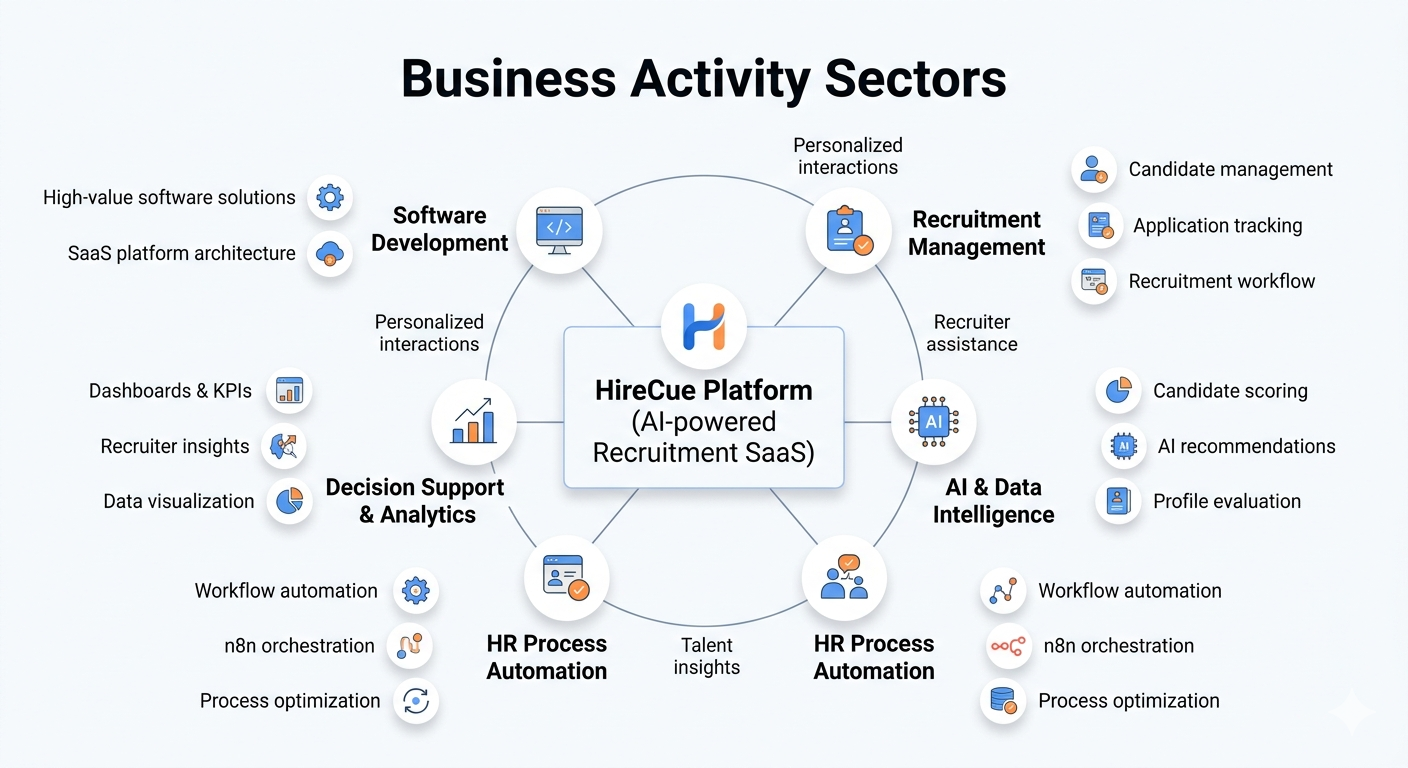
\includegraphics[width=0.75\textwidth]{Secteur}
\caption{Secteurs d'activite de l'entreprise d'accueil}
\end{figure}

\subsection{Organigramme de l'entreprise d'accueil}

L'organisation de l'entreprise peut etre lue a travers plusieurs poles complementaires. La direction generale assure l'orientation strategique des projets. Le pole developpement prend en charge la mise en oeuvre applicative et les integrations techniques. Le pole IA \& Data intervient sur les traitements intelligents, l'exploitation des donnees et la conception des sorties analytiques. Le pole produit veille a l'alignement entre la solution construite et le besoin metier. Enfin, le pole recrutement et relation client maintient le lien avec les usages du terrain et les attentes des utilisateurs finaux.

Une telle structuration favorise la coordination entre des dimensions qui, dans un projet comme \textit{HireCue}, ne peuvent pas etre traitees separement. Les evolutions techniques n'ont de valeur que si elles restent comprehensibles pour les utilisateurs et coherentes avec la realite du recrutement. Ce cadre a donc facilite le travail d'integration et d'amelioration realise pendant le stage.

\begin{figure}[H]
\centering
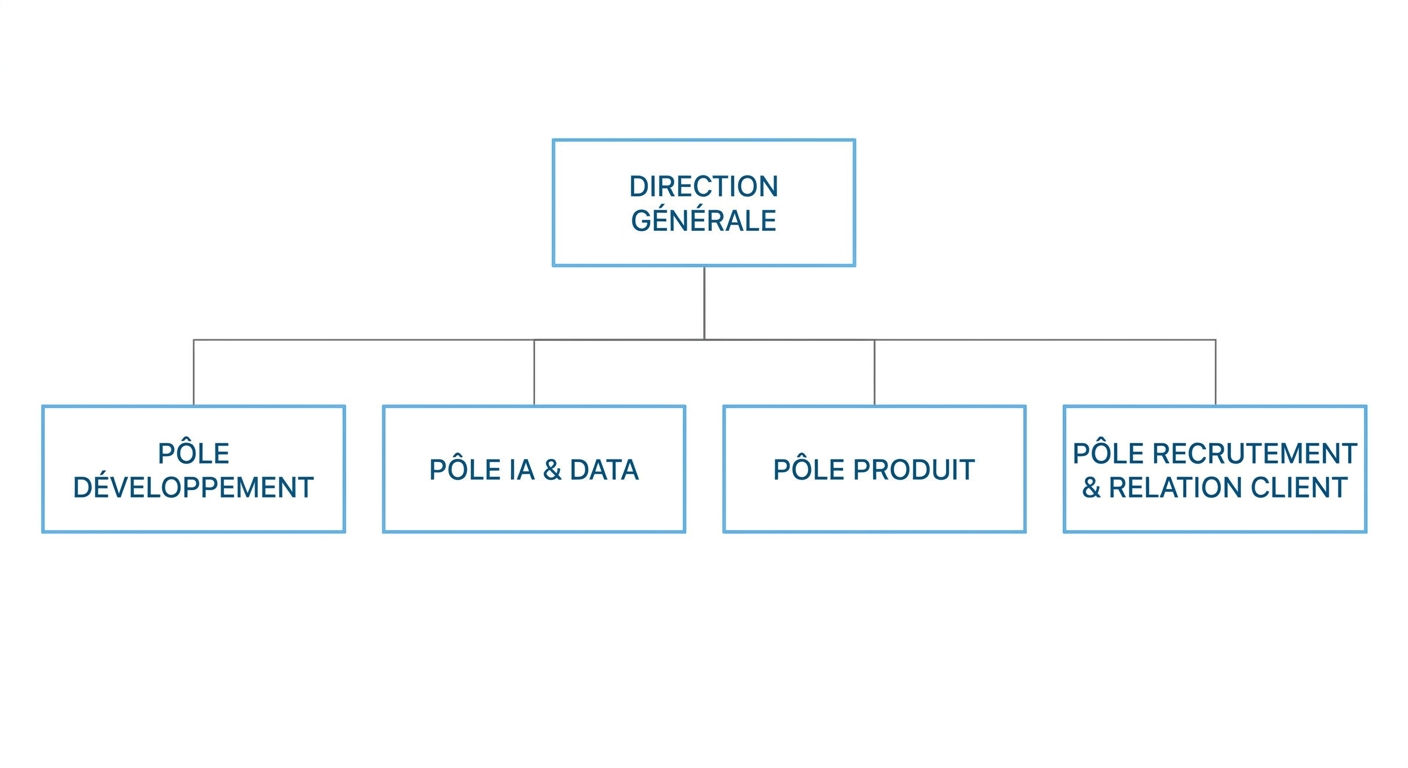
\includegraphics[width=0.80\textwidth]{Organigramme}
\caption{Organigramme fonctionnel de l'entreprise d'accueil}
\end{figure}

\section{Presentation du projet}

\textit{HireCue} est une plateforme SaaS de recrutement intelligente concue pour centraliser plusieurs etapes du processus de recrutement dans un meme environnement. Elle couvre deja la gestion des offres, le suivi des candidatures et differents mecanismes d'evaluation. Le travail realise pendant le stage ne consistait donc pas a construire un systeme a partir de zero, mais a faire evoluer un existant afin d'ameliorer la lisibilite des resultats et l'efficacite de certains parcours.

L'etude des repositories du projet montre une architecture articulee autour d'un frontend React, d'un backend Node.js et Express, d'une base MySQL pilotee via Sequelize, ainsi que de plusieurs services IA developpes en Python. Des mecanismes de cache, des traitements asynchrones et des workflows n8n viennent completer cet ensemble. Cette organisation n'a pas ete retenue de maniere abstraite : elle repond a la necessite d'introduire des fonctionnalites intelligentes sans fragiliser la plateforme principale ni alourdir excessivement les parcours existants.

Dans ce contexte, l'objectif du stage a porte sur des briques precises de \textit{HireCue}, notamment le rapport de score explicable, la roadmap de competences, le chatbot associe, les recommandations recruteur, la generation de questions personnalisees, le reengagement candidat et certaines integrations externes. Ces evolutions ont ete traitees parce qu'elles repondaient a des besoins reels de lisibilite, d'accompagnement et d'automatisation, tout en devant rester compatibles avec le fonctionnement deja en place.

\begin{figure}[H]
\centering

\includegraphics[width=0.42\textwidth]{hirecuelogo}
\caption{Logo de la plateforme HireCue}
\end{figure}

\section{Etude de l'existant}

L'etude de l'existant a d'abord consiste a situer \textit{HireCue} par rapport a des plateformes de recrutement numerique deja bien installees sur le marche, telles que TanitJobs et Keejob. Ces solutions occupent une place importante dans l'ecosysteme local du recrutement en ligne, en particulier pour la publication des offres, la visibilite des opportunites et la mise en relation entre entreprises et candidats.

Leur apport reste significatif, car elles repondent efficacement aux besoins de base : consulter des annonces, deposer un CV, postuler et permettre au recruteur de recevoir les candidatures. Cette logique reste cependant centree sur la diffusion et sur la centralisation des echanges initiaux, avec peu d'accent mis sur l'analyse approfondie du profil.

L'analyse menee dans le cadre du stage a montre que \textit{HireCue} se positionne sur un perimetre plus large. La plateforme ne cherche pas seulement a publier des offres, mais aussi a exploiter les donnees de candidature pour produire des scores, des explications, des recommandations, des roadmaps de progression et des tableaux de bord plus directement utiles a la decision. C'est dans ce passage d'un job board vers un outil d'orchestration et d'aide a la decision que se situe l'interet principal du projet.

\begin{figure}[H]
\centering

\includegraphics[width=0.35\textwidth]{tanitjob}
\caption{Logo de la plateforme TanitJobs}
\end{figure}

\begin{figure}[H]
\centering

\includegraphics[width=0.35\textwidth]{logo_keejob_light}
\caption{Logo de la plateforme Keejob}
\end{figure}

\begin{table}[H]
\centering
\begin{tabular}{|p{4cm}|p{3cm}|p{3cm}|p{3cm}|}
\hline
\rowcolor{headerblue}
\textbf{Critere} & \textbf{TanitJobs} & \textbf{Keejob} & \textbf{HireCue} \\
\hline
Type de plateforme & Job board et mise en relation & Job board et diffusion d'offres & Plateforme SaaS de recrutement intelligent \\
\hline
Fonctionnalites principales & Publication d'offres, consultation d'annonces, depot de CV & Offres d'emploi, recherche de profils, suivi basique des candidatures & Gestion des jobs, suivi des candidatures, rapports, recommandations et tableaux de bord \\
\hline
Utilisation de l'IA & Tres limitee ou non mise en avant & Tres limitee ou non mise en avant & Integree pour l'explication, la recommandation et l'assistance \\
\hline
Automatisation du recrutement & Faible & Faible a moderee & Presente via workflows, relances et integrations externes \\
\hline
Scoring des candidats & Non central & Limite & Oui, avec logique de score et rapports explicables \\
\hline
Personnalisation & Standardisee & Standardisee & Plus avancee selon le profil candidat et les besoins recruteur \\
\hline
Limites & Approche surtout orientee diffusion d'offres & Automatisation et aide a la decision encore limitees & Complexite technique plus elevee et besoin de maitrise des services IA \\
\hline
\end{tabular}
\caption{Comparaison entre TanitJobs, Keejob et HireCue}
\end{table}

Cette comparaison met en evidence un point important : les plateformes classiques couvrent correctement la phase d'entree dans le recrutement, mais elles accompagnent moins l'analyse approfondie du profil et la structuration de la decision. C'est precisement cet espace que \textit{HireCue} cherche a occuper.

\section{Critique de l'existant}

Les solutions classiques de recrutement rendent service lorsqu'il s'agit de diffuser des offres et de gerer un premier niveau d'interaction entre candidats et recruteurs. Leur limite apparait des que le volume de candidatures augmente ou que l'entreprise souhaite disposer d'une lecture plus fine des profils. Dans ce cas, le recruteur reste souvent contraint de reconstruire lui-meme une grande partie de l'analyse a partir de CV, de resultats disperses et d'informations peu homogenes.

L'une des limites observees concerne l'interpretation des scores et des evaluations. Dans de nombreux environnements, les resultats existent, mais ils ne sont pas toujours relies a une explication suffisamment claire pour etre utiles dans la decision. Cette difficulte a directement motive plusieurs evolutions apportees a \textit{HireCue}, notamment autour du score report et des sous-scores techniques, psychotechniques ou lies a la personnalite.

Une autre limite touche l'accompagnement du candidat. Les plateformes traditionnelles indiquent generalement l'etat d'une candidature, mais elles expliquent rarement les ecarts de competences ou les axes de progression. Dans le projet traite, cette dimension a ete jugee essentielle, ce qui justifie l'integration d'une roadmap de competences et d'un chatbot contextuel associe.

Enfin, le niveau d'automatisation reste souvent partiel. Les relances, le reengagement de candidats deja identifies, la personnalisation des entretiens ou l'exploitation d'integrations externes demandent encore beaucoup d'interventions manuelles. Ce constat ne remet pas en cause l'utilite des plateformes existantes, mais il montre qu'elles laissent une marge d'amelioration reelle pour une solution comme \textit{HireCue}, dont l'ambition est d'assister plus directement le pilotage du recrutement.

\section{Problematique}

Le recrutement moderne produit une quantite importante de donnees provenant de sources diverses : CV, offres, resultats de tests, historiques de candidature, interactions utilisateurs et sorties generees par des services intelligents. L'enjeu ne se limite donc plus a collecter ces informations. Il consiste plutot a les organiser, les interpreter et les restituer sous une forme exploitable par les differents acteurs.

Dans ce cadre, les recruteurs ont besoin d'outils capables de reduire le tri manuel, de faire ressortir les candidatures les plus pertinentes et d'expliquer les resultats proposes. Les candidats, quant a eux, attendent un suivi plus lisible, des retours plus concrets et une meilleure comprehension de leur positionnement par rapport a une offre.

L'introduction de l'intelligence artificielle peut repondre a une partie de ces attentes, a condition qu'elle soit integree de facon maitrisee. Un systeme trop opaque ou trop deconnecte du besoin metier risquerait d'ajouter de la complexite au lieu d'ameliorer le processus. C'est pourquoi la question n'etait pas simplement d'ajouter de l'IA a une plateforme existante, mais de l'inserer de maniere utile, explicable et techniquement soutenable.

La problematique centrale du projet peut ainsi etre formulee comme suit : comment faire evoluer une plateforme de recrutement existante vers une solution plus intelligente, plus automatisee et plus explicable, capable d'assister les recruteurs dans l'evaluation des candidatures tout en offrant aux candidats des retours personnalises et exploitables ?

\section{Solution proposee}

La solution retenue pendant le stage a consiste a enrichir \textit{HireCue} par des fonctionnalites d'analyse, d'assistance et d'automatisation construites autour du socle deja present. Le choix n'a pas ete de remplacer les mecanismes metier existants, mais de les completer par des services apportant plus de clarte dans les resultats et plus de fluidite dans les parcours.

Concretement, le travail a porte sur plusieurs axes complementaires. Le premier concerne l'explicabilite, avec l'amelioration du rapport de score afin de rendre les resultats plus lisibles pour le candidat comme pour le recruteur. Le deuxieme porte sur l'accompagnement candidat, a travers la generation d'une roadmap de competences et l'ajout d'un chatbot RAG permettant d'obtenir des reponses contextualisees sur cette progression. Le troisieme vise l'aide a la decision cote recruteur, avec des recommandations de candidats, des questions personnalisees pour l'entretien et des elements d'analyse plus directement exploitables dans les dashboards.

Le stage a egalement porte sur des besoins plus operationnels, comme le reengagement de candidats, la gestion de certaines notifications, le suivi de quotas IA, l'usage du cache pour limiter les recalculs couteux et l'integration de workflows n8n pour l'import d'offres externes, le sourcing LinkedIn et d'autres traitements transverses. Ce volet etait important, car une fonctionnalite utile en demonstration ne l'est pas necessairement en production si elle reste couteuse, peu tra\c cable ou difficile a integrer. L'ensemble des choix retenus poursuit donc une meme logique : rendre la plateforme plus utile dans un contexte reel, sans perdre la maitrise technique des traitements engages.

\section{Methodologie}

La demarche adoptee repose sur une progression iterative, adaptee a l'evolution d'une plateforme deja en service. Ce choix etait necessaire, car le projet ne consistait pas a produire un prototype isole, mais a intervenir sur un systeme comportant deja des interfaces, des services metier, une base de donnees, des integrations externes et plusieurs dependances techniques.

Une approche progressive etait plus adaptee a la realite du projet. Elle permettait de comprendre l'existant avant d'y ajouter de nouvelles briques, de limiter les regressions et de verifier la coherence des integrations au fur et a mesure. Elle repondait aussi a la nature hybride du travail mene, situe a l'intersection du developpement logiciel classique, des services IA et des workflows d'automatisation.

\subsection{Phase d'analyse}

La premiere phase du travail a consiste a etudier l'existant de facon detaillee. Cette etape a porte sur l'organisation des repositories, la structure du frontend, les services backend, les routes exposees, les modeles de donnees et les interactions avec les services externes. Elle a permis d'identifier les briques deja disponibles dans \textit{HireCue}, mais aussi les zones dans lesquelles les evolutions etaient les plus pertinentes.

Cette analyse a notamment mis en evidence plusieurs besoins concrets : mieux expliquer les scores, proposer une roadmap plus exploitable pour le candidat, structurer les recommandations recruteur, encadrer l'usage des services IA par des quotas et fiabiliser certaines integrations externes. Elle a aussi permis de mieux comprendre les contraintes de l'architecture, en particulier la coexistence entre traitements synchrones, workflows asynchrones, cache applicatif et appels a des services IA distincts.

\subsection{Phase de conception et d'integration}

La seconde phase a consiste a traduire ces constats en evolutions concretes au sein de la plateforme. Les interfaces ont ete adaptees pour exposer les nouvelles informations de maniere plus claire. Cote backend, les services ont ete organises pour orchestrer les appels, persister les resultats, reutiliser les donnees deja calculees lorsque cela etait possible et maintenir des echanges coherents avec les composants externes.

Une attention particuliere a ete accordee a des aspects souvent determinants en contexte reel : la journalisation, la gestion des erreurs, les quotas IA, le cache, les traitements asynchrones et la persistance des sorties generees. Ces choix n'ont pas seulement une justification technique. Ils conditionnent aussi la stabilite de la plateforme et la possibilite de faire evoluer les modules intelligents sans degrader l'experience utilisateur.

\subsubsection{Principe directeur}

Le principe directeur de cette phase a ete de rechercher un equilibre entre richesse fonctionnelle et maitrise de la complexite. Les services intelligents devaient apporter une aide tangible, mais sans produire des sorties opaques ou difficilement integrables. De la meme maniere, les automatisations devaient reduire certaines charges manuelles sans masquer les etapes importantes du processus de recrutement. Cette orientation a guide les choix realises sur \textit{HireCue} pendant tout le stage.

\subsection{Choix des methodologies adoptees}

Le projet combine deux dimensions qui ne relevent pas exactement des memes pratiques. La premiere correspond au developpement logiciel de la plateforme, avec ses besoins de planification, d'integration et de validation progressive. La seconde concerne les modules IA et LLM, qui necessitent davantage de vigilance sur les donnees d'entree, la qualite des sorties, les formats retournes et la pertinence metier des resultats.

Pour cette raison, deux references methodologiques ont ete retenues. La dimension applicative s'appuie sur Agile Scrum, plus adaptee au developpement iteratif des interfaces et des services. Les modules IA, quant a eux, sont mieux encadres par une logique proche de CRISP-DM, qui permet de relier plus explicitement le besoin metier, les donnees mobilisees, la generation des sorties et leur evaluation.

\begin{table}[H]
\centering
\renewcommand{\arraystretch}{1.3}
\begin{tabular}{|p{4cm}|p{4cm}|p{6cm}|}
\hline
\rowcolor{headerblue}
\textbf{Domaine} & \textbf{Methodologie adoptee} & \textbf{Justification} \\
\hline
Developpement Frontend / Backend & Agile Scrum & Permet un developpement iteratif, flexible et adapte a l'evolution progressive des fonctionnalites du systeme. \\
\hline
Developpement IA / LLM incluant le chatbot RAG & CRISP-DM & Methodologie adaptee aux projets de data science et d'intelligence artificielle, structuree autour de la comprehension metier, des donnees, de la modelisation, de l'evaluation et du deploiement. \\
\hline
\end{tabular}
\caption{Methodologies adoptees selon les domaines du projet}
\end{table}

\subsection{Methodologie Agile Scrum pour le developpement logiciel}

La reference a Scrum se justifie par le caractere progressif des evolutions apportees a \textit{HireCue}. Les fonctionnalites n'ont pas ete traitees comme un bloc unique, mais comme un ensemble d'ameliorations successives : score report, dashboards, roadmap, chatbot, recommandations, notifications et automatisations. Une telle organisation facilite les ajustements, permet de prioriser les taches a plus forte valeur et rend plus simple la prise en compte des retours au fur et a mesure.

Dans le cadre du stage, cette logique a surtout ete utile pour articuler des travaux de nature differente. Certaines taches relevaient du frontend, d'autres du backend, d'autres encore de l'integration de services IA ou de workflows n8n. Une progression iterative etait donc plus realiste qu'une planification strictement lineaire.

\subsubsection{Les roles Scrum}

Dans Scrum, le \textit{Product Owner} porte le besoin metier et priorise les fonctionnalites selon la valeur attendue. Ce role est important dans un projet comme \textit{HireCue}, car toutes les evolutions possibles n'ont pas le meme impact sur le recrutement.

Le \textit{Scrum Master} veille au bon deroulement du cadre de travail, aide a lever les blocages et facilite la coordination entre les participants. Son role est moins de diriger que de maintenir des conditions favorables a une progression reguliere.

L'equipe de developpement rassemble enfin les profils qui transforment ces besoins en fonctionnalites concretes. Dans le cas present, cette logique de collaboration est particulierement pertinente, car les evolutions touchent simultanement aux interfaces, aux services metier, aux integrations externes et aux modules intelligents.

\begin{figure}[H]
\centering
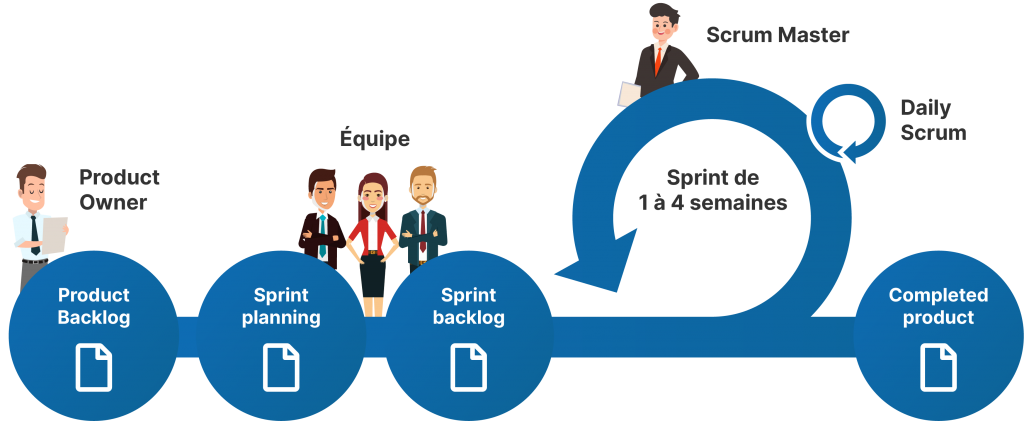
\includegraphics[width=0.75\textwidth]{scrum}
\caption{Cycle de vie de la methodologie Scrum}
\end{figure}

\subsection{Methodologie CRISP-DM pour les modules IA}

Pour les modules d'intelligence artificielle, la reference a CRISP-DM apparait plus appropriee. Les traitements mis en place dans \textit{HireCue} ne peuvent pas etre juges uniquement sur leur faisabilite technique. Ils doivent aussi etre evalues selon la qualite des donnees exploitees, la pertinence des sorties produites et leur adequation avec les usages vises.

Dans ce projet, cette exigence est visible a plusieurs niveaux. Un score explicable n'a d'interet que s'il repose sur des donnees coherentes et s'il fournit une justification comprehensible. Une roadmap n'est utile que si elle reste realiste par rapport au profil du candidat et au poste cible. De meme, un chatbot contextuel ne peut etre integre que si ses reponses restent suffisamment alignees avec le contenu de la roadmap et avec les contraintes de la plateforme.

Les etapes de CRISP-DM permettent d'encadrer cette logique. La phase de \textit{Business Understanding} consiste a clarifier le besoin reel, par exemple expliquer un score ou assister un candidat dans sa progression. La phase de \textit{Data Understanding} porte sur les informations disponibles : CV, scores, resultats d'evaluation, donnees de poste ou historiques de candidature. La phase de \textit{Data Preparation} vise ensuite a structurer ces donnees pour qu'elles puissent alimenter correctement les services intelligents.

La phase de \textit{Modeling} correspond a l'utilisation ou a l'orchestration des modeles mobilises pour generer les sorties attendues. La phase d'\textit{Evaluation} est essentielle pour verifier la coherence des contenus produits, leur format et leur utilite metier. Enfin, la phase de \textit{Deployment} concerne l'integration de ces services dans \textit{HireCue}, avec les contraintes de cache, de quotas, de persistance et de robustesse propres a un environnement applicatif.

Cette demarche a ete particulierement utile pour les modules lies au score report, a la roadmap de competences, au chatbot associe, aux recommandations recruteur et aux questions personnalisees. Elle permet de mieux justifier les choix retenus et d'encadrer l'usage de l'IA dans une logique de service plutot que de demonstration technologique.

\begin{figure}[H]
\centering
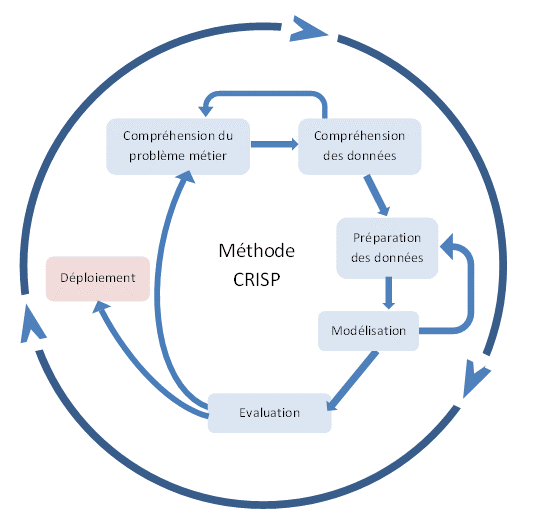
\includegraphics[width=0.75\textwidth]{mthode-crisp}
\caption{Cycle de vie de la methodologie CRISP-DM}
\end{figure}

\section*{Conclusion}
\addcontentsline{toc}{section}{Conclusion}

Ce chapitre a permis de situer le projet dans son cadre organisationnel et technique, puis de montrer en quoi l'evolution de \textit{HireCue} repond a un besoin reel du recrutement numerique. L'analyse de l'existant a fait ressortir des limites en matiere d'explicabilite, de personnalisation et d'automatisation, ce qui justifie les orientations retenues pendant le stage.

La problematique et la demarche methodologique apparaissent ainsi de facon plus coherente. Cette base permet d'aborder, dans le chapitre suivant, les besoins de la plateforme et la planification du projet avec une lecture plus precise des objectifs poursuivis.

\chapter{Sp\'ecifications des besoins et Planification du projet}

\section*{Introduction}
\addcontentsline{toc}{section}{Introduction}

Ce chapitre formalise les besoins du projet \textit{HireCue} et rassemble les principaux elements ayant structure son evolution pendant le stage. L'accent est d'abord mis sur les acteurs du systeme, puis sur les besoins fonctionnels et non fonctionnels ainsi que sur le backlog produit. La lecture se prolonge ensuite par l'architecture globale de l'application, les diagrammes UML utiles a la comprehension du systeme et l'etude des logiciels et des technologies mobilises.

\section{Sp\'ecifications des besoins}

La specification des besoins permet de definir les fonctionnalites attendues de la plateforme \textit{HireCue} ainsi que les contraintes de qualite qui encadrent leur mise en oeuvre. Dans un projet de recrutement intelligent, cette etape est importante, car elle relie les attentes des utilisateurs, les choix techniques et les objectifs metier.

\subsection{Identification des acteurs}

Dans un systeme d'information, un acteur designe toute entite humaine ou technique qui interagit avec l'application ou participe a l'execution de certaines fonctions. Dans \textit{HireCue}, cette notion ne se limite pas aux utilisateurs finaux, puisque plusieurs services d'IA, workflows d'automatisation et systemes externes interviennent aussi dans le traitement des donnees et dans l'execution du processus de recrutement.

\begin{table}[H]
\centering
\renewcommand{\arraystretch}{1.3}
\begin{tabular}{|p{4cm}|p{10cm}|}
\hline
\rowcolor{headerblue}
\textbf{Acteur} & \textbf{Role principal} \\
\hline
Candidat & Consulte les offres, suit ses candidatures, accede au rapport de score, visualise la roadmap de competences et interagit avec le chatbot associe a sa progression. \\
\hline
Recruteur & Gere les offres, consulte les profils, analyse les scores, exploite les recommandations IA, prepare les entretiens et utilise les outils de reengagement et de sourcing. \\
\hline
Administrateur & Supervise le fonctionnement global de la plateforme, controle certains traitements transverses et intervient sur la gestion generale des integrations et des utilisateurs. \\
\hline
Service IA / LLM & Produit certaines sorties d'analyse ou de generation, comme les explications de score, les recommandations, les roadmaps, les questions personnalisees et les reponses contextuelles du chatbot. \\
\hline
Workflows n8n & Orchestrent plusieurs automatisations, notamment l'import d'offres externes, certains flux de sourcing et des traitements relies aux integrations externes. \\
\hline
Systeme externe LinkedIn / PhantomBuster & Fournit un support aux operations de sourcing et a certains flux externes relies a la recherche de profils ou a la circulation d'informations entre plateformes. \\
\hline
\end{tabular}
\caption{Identification des acteurs du systeme}
\end{table}

\subsection{Besoins fonctionnels}

Les besoins fonctionnels correspondent aux services que la plateforme doit rendre aux differents acteurs du recrutement. Dans le cas de \textit{HireCue}, ils depassent la gestion classique des offres et des candidatures. Ils couvrent aussi l'explicabilite des scores, l'accompagnement du candidat, l'assistance au recruteur et l'automatisation de plusieurs operations transverses. Cette extension fonctionnelle n'a pas ete definie de maniere theorique. Elle repond a des besoins identifies pendant le stage, en particulier la clarte des evaluations, la lisibilite des parcours et l'exploitation plus efficace des donnees deja presentes dans la plateforme. C'est pourquoi \textit{HireCue} doit assurer l'authentification et la gestion des roles, la gestion des offres et des candidatures, la consultation d'un rapport de score explicable, la generation de recommandations IA cote recruteur, la production de questions personnalisees pour l'entretien, la construction d'une roadmap de competences, la mise a disposition d'un chatbot RAG, la gestion des notifications et du reengagement, l'import d'offres via \textit{n8n}, le sourcing LinkedIn, le suivi des quotas IA ainsi que la visualisation de tableaux de bord adaptes aux profils utilisateur.

\begin{figure}[H]
\centering
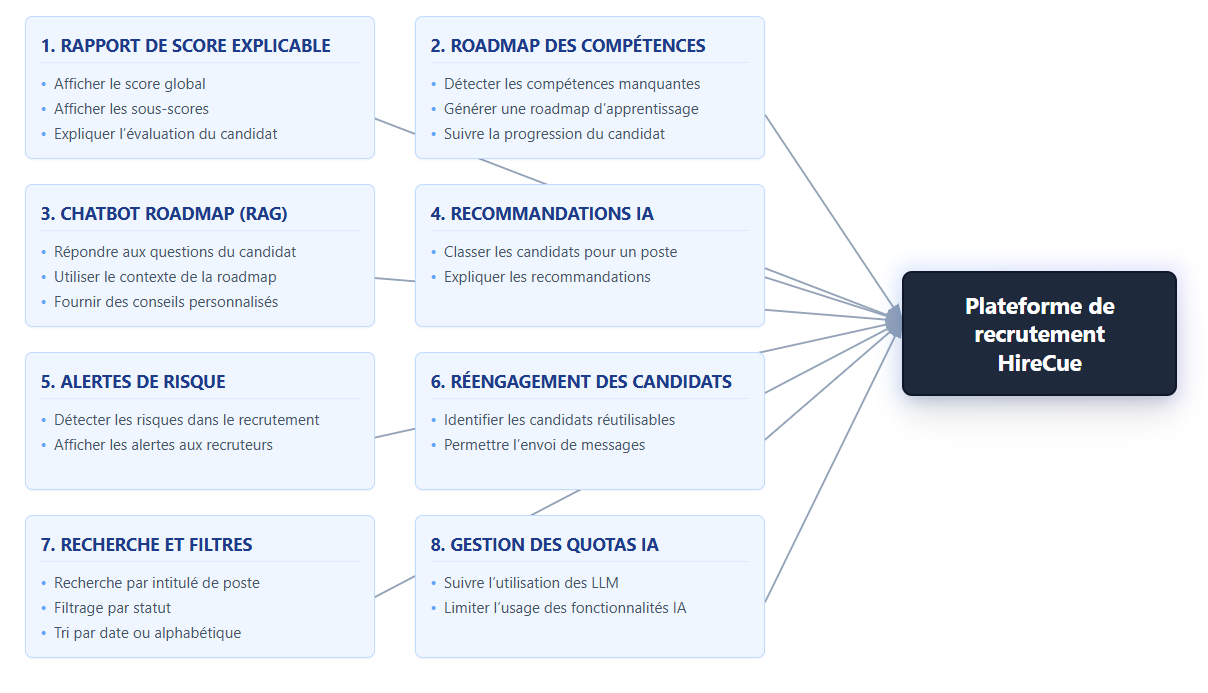
\includegraphics[width=0.9\textwidth]{besoinsfonctionnels}
\caption{Besoins fonctionnels de la plateforme HireCue}
\end{figure}

\subsection{Besoins non fonctionnels}

Au-dela des fonctionnalites attendues, \textit{HireCue} doit respecter plusieurs exigences de qualite liees a son usage reel et a la nature heterogene de son architecture. La \textbf{performance} est importante pour garantir des temps de reponse convenables lors de la consultation des dashboards, des rapports ou des parcours candidats. La \textbf{securite} reste essentielle en raison de la sensibilite des donnees traitees et de la multiplicite des roles. La \textbf{fiabilite} et la \textbf{maintenabilite} permettent d'assurer un comportement coherent de la plateforme malgre les interactions entre frontend, backend, services IA et integrations externes. La \textbf{scalabilite} doit permettre d'absorber une hausse du volume de candidatures et de traitements asynchrones. L'\textbf{ergonomie} contribue a rendre les resultats lisibles pour les utilisateurs, tandis que la \textbf{disponibilite}, la \textbf{tracabilite}, la \textbf{gestion des erreurs} et le \textbf{controle des quotas IA} conditionnent la robustesse globale du systeme et la maitrise des traitements couteux.

\begin{figure}[H]
\centering
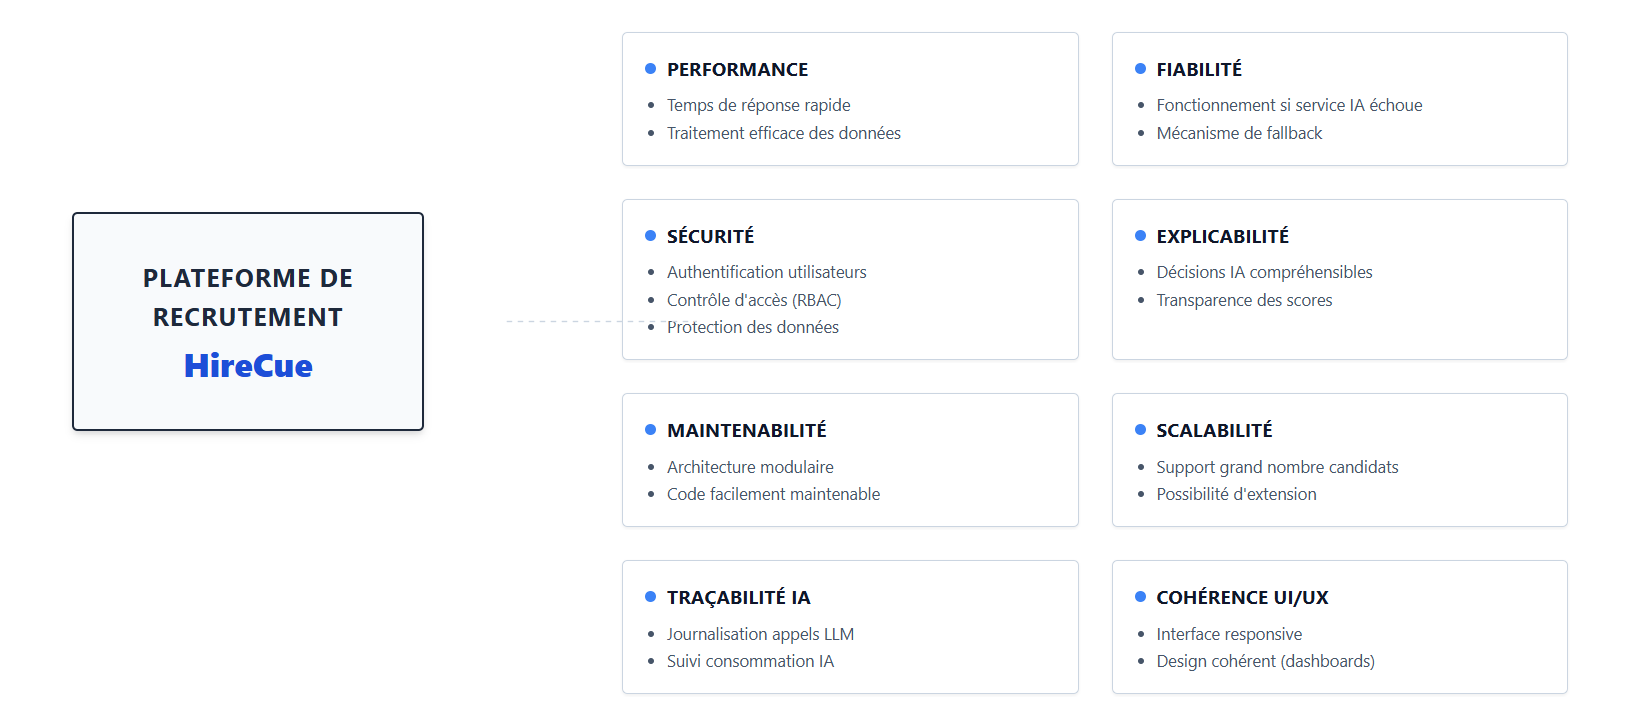
\includegraphics[width=0.9\textwidth]{Besoinsnonfonctionnels}
\caption{Besoins non fonctionnels de la plateforme HireCue}
\end{figure}

\subsection{Backlog produit}

Le backlog produit regroupe les principales fonctionnalites a developper, a integrer ou a ameliorer dans le cadre du projet. Il permet d'organiser les priorites en fonction de la valeur metier attendue, de la complexite technique et des dependances existantes entre les differentes briques de la plateforme. Dans le cas de \textit{HireCue}, cette priorisation etait necessaire, car les evolutions ne pouvaient pas etre traitees independamment les unes des autres : l'explicabilite du score, l'accompagnement candidat, les recommandations et les integrations externes devaient progresser de maniere coherente.

\begin{table}[H]
\centering
\small
\renewcommand{\arraystretch}{1.25}
\begin{tabular}{|p{1.2cm}|p{4.5cm}|p{2.5cm}|p{2cm}|p{2cm}|}
\hline
\rowcolor{headerblue}
\textbf{ID} & \textbf{Fonctionnalite} & \textbf{ID User Story} & \textbf{Complexite} & \textbf{Priorite} \\
\hline
F01 & Authentification et gestion des roles & US01 & Moyenne & Haute \\
\hline
F02 & Rapport de score explicable & US02 & Elevee & Haute \\
\hline
F03 & Skill Gap Roadmap & US03 & Elevee & Haute \\
\hline
F04 & Chatbot RAG & US04 & Elevee & Haute \\
\hline
F05 & Recommandations IA & US05 & Elevee & Haute \\
\hline
F06 & Questions personnalisees & US06 & Moyenne & Moyenne \\
\hline
F07 & Reengagement candidat & US07 & Moyenne & Moyenne \\
\hline
F08 & Notifications & US08 & Moyenne & Moyenne \\
\hline
F09 & Import d'offres externes via n8n & US09 & Elevee & Haute \\
\hline
F10 & Sourcing LinkedIn via PhantomBuster & US10 & Elevee & Moyenne \\
\hline
F11 & Dashboard candidat & US11 & Moyenne & Haute \\
\hline
F12 & Dashboard recruteur & US12 & Moyenne & Haute \\
\hline
F13 & Suivi des quotas IA & US13 & Moyenne & Haute \\
\hline
F14 & Journalisation et cache & US14 & Moyenne & Haute \\
\hline
\end{tabular}
\caption{Backlog produit du projet HireCue}
\end{table}
\normalsize

\section{Architecture logique et physique globale de l'application}

L'architecture globale permet de comprendre la maniere dont les composants techniques de \textit{HireCue} sont organises et coordonnes. Elle met en evidence les relations entre l'interface utilisateur, la logique metier, les services IA, la base de donnees et les outils d'automatisation mobilises dans le projet. Cette lecture est importante, car une partie essentielle du stage a consiste a faire evoluer des briques deja existantes sans rompre l'equilibre d'ensemble de la plateforme.

\subsection{Architecture physique de l'application}

L'architecture physique de \textit{HireCue} repose sur une organisation distribuee dans laquelle plusieurs briques cooperent par des echanges API. L'utilisateur accede a la plateforme depuis un poste client a travers un navigateur web. Les interfaces sont portees par un frontend React, qui communique avec un backend principal developpe en Node.js et Express. Ce backend centralise la logique metier, l'acces aux donnees et l'orchestration des traitements. Il interagit avec une base de donnees MySQL pour la persistence, avec des services IA Python / LLM pour certaines generations et analyses, ainsi qu'avec des workflows \textit{n8n} pour plusieurs automatisations. Des services externes, tels que LinkedIn et PhantomBuster, interviennent egalement dans certains flux de sourcing ou d'integration. L'ensemble des communications se fait principalement via des APIs REST, ce qui facilite l'interconnexion entre les briques tout en conservant une separation nette des responsabilites.

\begin{figure}[H]
\centering
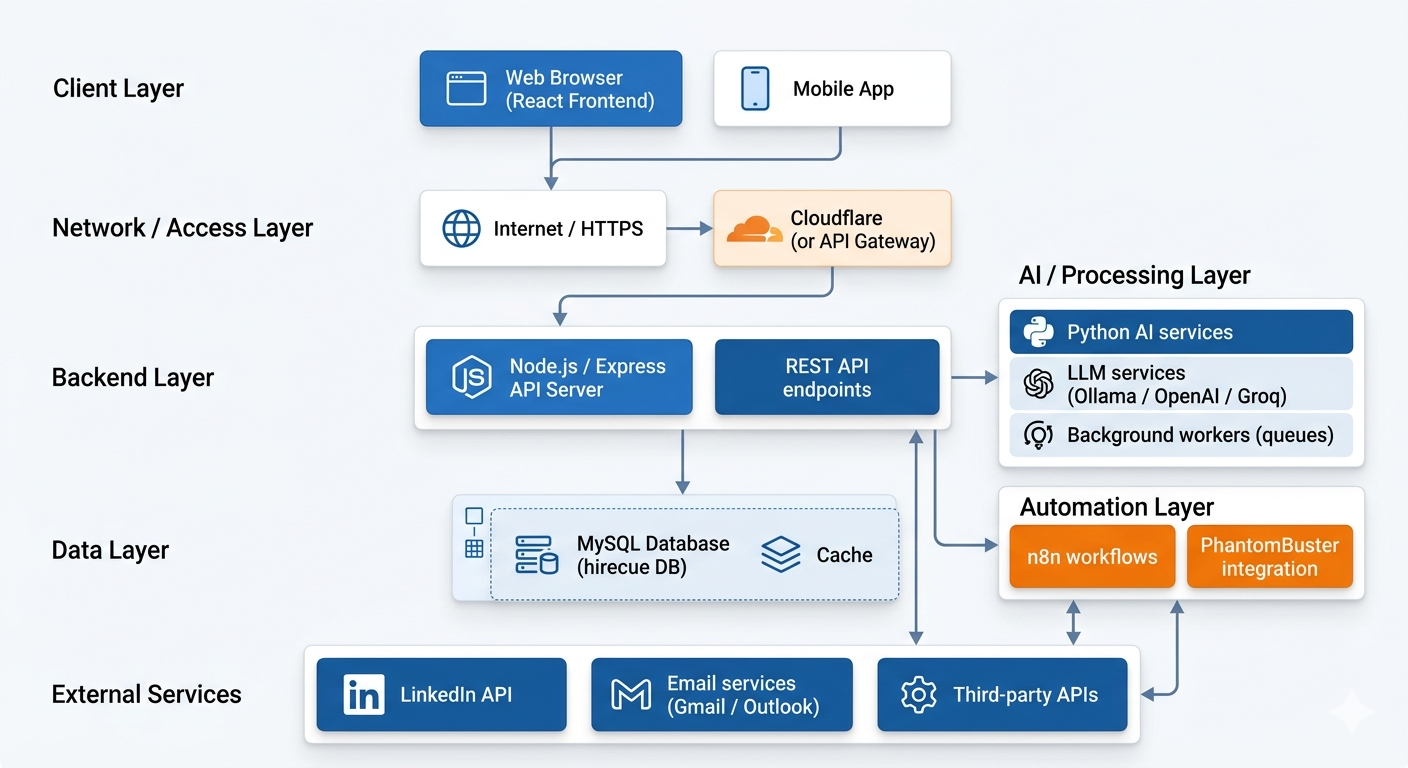
\includegraphics[width=\textwidth]{Architecture_physique}
\caption{Architecture physique de l'application HireCue}
\end{figure}

\subsection{Architecture logique de l'application}

Sur le plan logique, \textit{HireCue} peut etre decomposee en plusieurs couches complementaires. La \textbf{couche presentation} regroupe les interfaces React destinees au candidat, au recruteur et a l'administrateur. La \textbf{couche metier} est portee par le backend Node.js / Express et prend en charge les regles de gestion, les routes applicatives, l'orchestration des parcours et la coordination avec les autres services. La \textbf{couche services IA} rassemble les traitements utilises pour expliquer les scores, generer les roadmaps, produire des recommandations ou assister l'entretien. La \textbf{couche donnees} repose sur MySQL et assure la persistence des utilisateurs, des candidatures, des scores, des roadmaps, des notifications et des historiques associes. La \textbf{couche orchestration et automatisation} est principalement assuree par \textit{n8n} et par certains traitements asynchrones relies a la plateforme. Enfin, la \textbf{couche integration externe} couvre les interactions avec LinkedIn, PhantomBuster et d'autres sources externes mobilisees pour le sourcing ou l'import d'offres.

\begin{figure}[H]
\centering
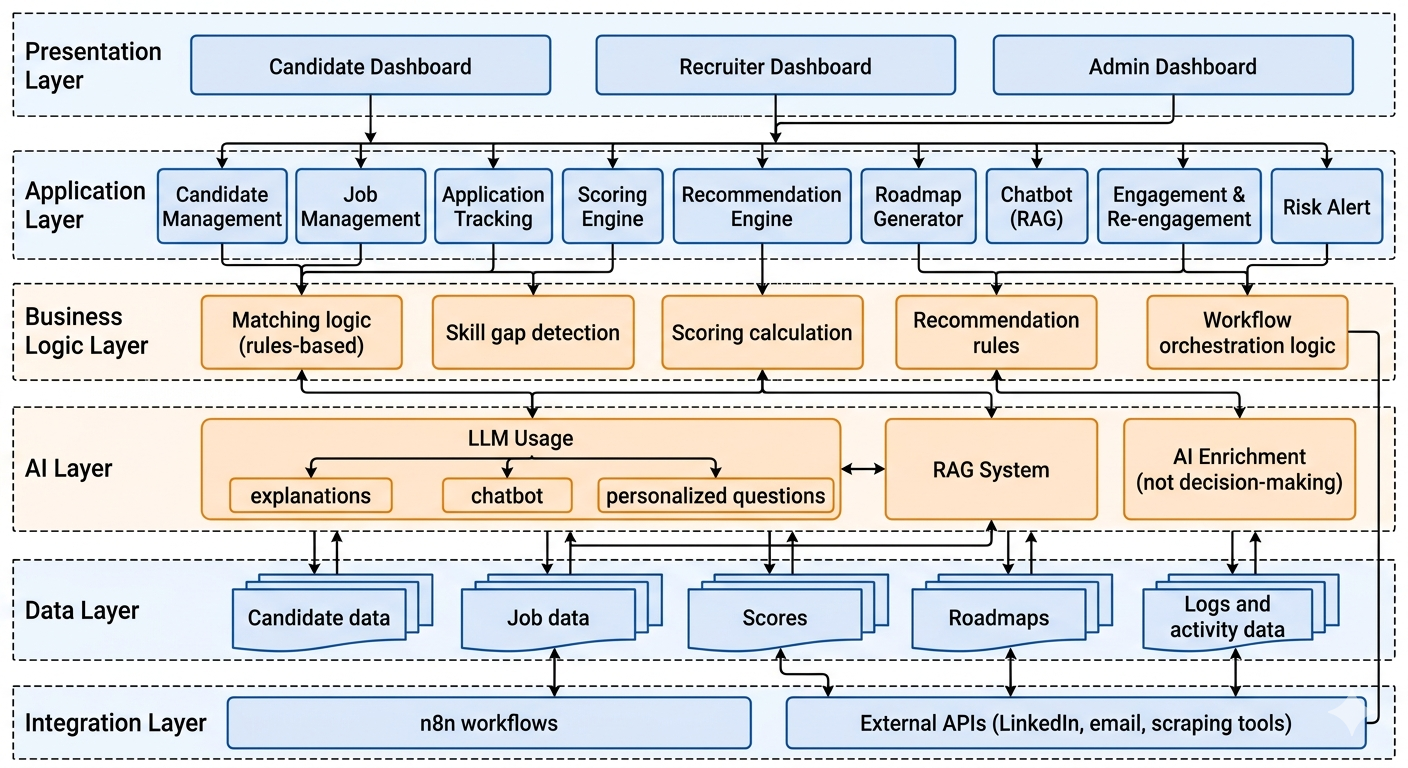
\includegraphics[width=\textwidth]{Architecture_logique}
\caption{Architecture logique de l'application HireCue}
\end{figure}

\section{Diagrammes UML}

Les diagrammes UML facilitent la comprehension du systeme en offrant une representation synthetique des interactions, des responsabilites et des principales entites manipulees par la plateforme.

\subsection{Diagramme de cas d'utilisation global}

Le diagramme de cas d'utilisation global montre les principales interactions entre les acteurs et les fonctionnalites majeures de \textit{HireCue}. Il fait apparaitre les roles du candidat, du recruteur, de l'administrateur, des services IA et des workflows externes. Cette representation permet de visualiser les cas d'utilisation centraux du projet, notamment la consultation des scores, la generation d'une roadmap, l'exploitation des recommandations, la gestion des offres, l'import d'offres externes et les operations de sourcing.

\begin{figure}[H]
\centering
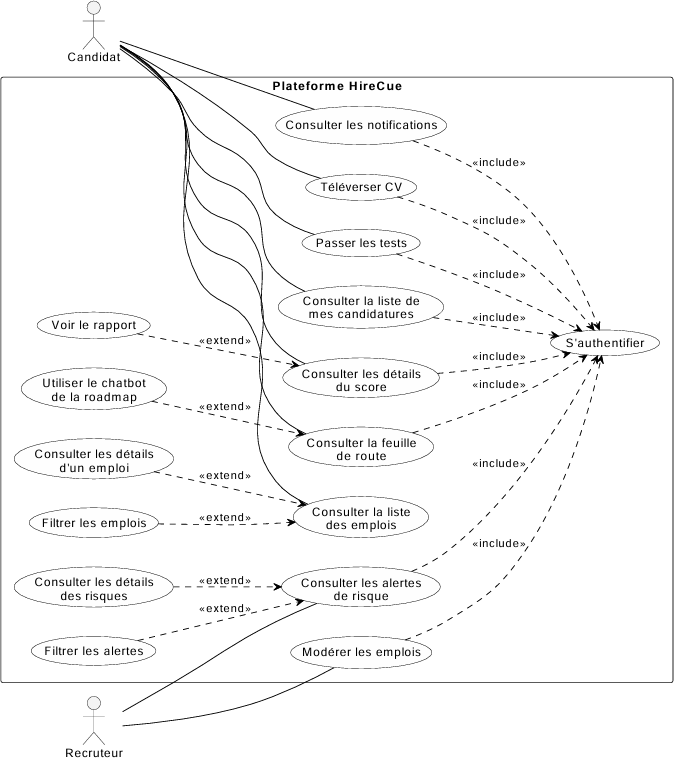
\includegraphics[width=\textwidth]{Casdutilisation_globale}
\caption{Diagramme de cas d'utilisation global de la plateforme HireCue}
\end{figure}

\subsection{Diagramme des classes d'analyse global}

Le diagramme des classes d'analyse represente les principales entites metier manipulees par la plateforme et les relations qu'elles entretiennent entre elles. Dans le cas de \textit{HireCue}, il permet de structurer des entites telles que l'utilisateur, le candidat, le recruteur, l'offre, la candidature, le score, la roadmap, la notification, le workflow et la recommandation. Ce diagramme contribue a clarifier l'organisation des donnees et a mieux comprendre la maniere dont les composants fonctionnels s'articulent au sein du systeme.

\IfFileExists{diagramme_classe.png}{
\begin{figure}[H]
\centering
\includegraphics[width=\textwidth]{diagramme_classe}
\caption{Diagramme des classes d'analyse global}
\end{figure}
}{
\begin{figure}[H]
\centering
\includegraphics[width=\textwidth]{"diagramme de classe"}
\caption{Diagramme des classes d'analyse global}
\end{figure}
}

\section{\'Etude des outils}

Cette partie presente les logiciels et les technologies mobilises dans le projet, ainsi que les principaux criteres ayant oriente leur choix. L'objectif est de montrer que les outils retenus repondent a des besoins concrets de developpement, d'integration, d'automatisation et d'exploitation des services intelligents.

\subsection{Logiciels utilises}

Le developpement et l'integration de \textit{HireCue} ont mobilise plusieurs logiciels intervenant a differentes etapes du travail, depuis l'edition du code jusqu'aux tests, au versionnement, a l'automatisation et a la redaction du rapport. Leur usage n'est pas uniquement lie au confort de developpement ; il repond aussi a la necessite de verifier les integrations, de suivre les traitements et de maintenir une base de travail suffisamment stable tout au long du stage.

\begin{table}[H]
\centering
\small
\renewcommand{\arraystretch}{1.4}
\begin{tabular}{|m{2.5cm}|p{3.5cm}|p{8cm}|}
\hline
\rowcolor{headerblue}
\textbf{Logo} & \textbf{Nom} & \textbf{Information} \\
\hline
-- & Visual Studio Code & Environnement de developpement utilise pour editer le code frontend, backend et certains services associes au projet. \\
\hline
-- & Git / GitHub & Outils utilises pour le versionnement du code, le suivi des modifications et la coordination du travail sur les repositories. \\
\hline
-- & Postman & Logiciel de test d'API employe pour verifier les routes backend et certaines integrations externes. \\
\hline
-- & Docker & Outil utilise pour encapsuler ou executer certaines briques techniques du projet dans un environnement controle. \\
\hline
-- & n8n & Plateforme d'automatisation mobilisee pour l'orchestration de workflows, l'import d'offres et certains flux externes. \\
\hline
-- & MySQL Workbench / phpMyAdmin & Outils de consultation et d'administration de la base de donnees utilises pour verifier les structures et le contenu des tables. \\
\hline
-- & Overleaf & Environnement de redaction LaTeX adapte a la preparation, a la structuration et a la mise en forme du rapport PFE. \\
\hline
-- & PhantomBuster & Outil utilise dans certains workflows de sourcing LinkedIn et d'exploitation de profils externes. \\
\hline
-- & Power BI & Outil cite dans le contexte projet comme piste ou environnement de visualisation a verifier selon les usages effectifs. \\
\hline
\end{tabular}
\caption{Logiciels utilises dans le projet}
\end{table}
\normalsize

\subsection{Technologies utilisees}

Le projet \textit{HireCue} s'appuie sur un ensemble de technologies complementaires, choisies pour couvrir les besoins d'interface, de logique metier, de persistence, de services intelligents et d'integration entre composants. Cette combinaison technologique reflete directement la nature du travail realise, qui demandait a la fois une interface exploitable, un backend robuste, des integrations externes et des briques d'IA encadrees.

\begin{table}[H]
\centering
\small
\renewcommand{\arraystretch}{1.4}
\begin{tabular}{|m{2.5cm}|p{3.5cm}|p{8cm}|}
\hline
\rowcolor{headerblue}
\textbf{Logo} & \textbf{Nom} & \textbf{Information} \\
\hline
-- & React.js & Bibliotheque frontend utilisee pour construire les interfaces de la plateforme et structurer les parcours utilisateur. \\
\hline
-- & Node.js & Environnement d'execution JavaScript retenu pour le backend principal de l'application. \\
\hline
-- & Express.js & Framework backend employe pour structurer les routes, les services metier et les APIs du projet. \\
\hline
-- & MySQL & Systeme de gestion de base de donnees utilise pour la persistence des informations metier. \\
\hline
-- & Sequelize & ORM utilise pour simplifier l'acces aux donnees et la manipulation des tables MySQL depuis le backend. \\
\hline
-- & Python & Langage mobilise pour plusieurs services IA et certaines briques de generation ou d'analyse. \\
\hline
-- & Ollama / LLM & Outils utilises pour certaines generations textuelles et pour l'integration de traitements fondes sur des modeles de langage. \\
\hline
-- & RAG & Approche utilisee pour structurer le chatbot lie a la roadmap et contextualiser certaines reponses. \\
\hline
-- & REST API & Mode de communication principal entre frontend, backend, services IA et integrations externes. \\
\hline
-- & Socket.IO & Technologie citee dans le contexte projet comme composant eventuel de communication temps reel, a mobiliser selon les besoins de l'application. \\
\hline
-- & Firebase Authentication & Solution citee dans le contexte projet parmi les briques techniques a considerer selon l'architecture et les usages de l'authentification. \\
\hline
\end{tabular}
\caption{Technologies utilisees dans le projet}
\end{table}
\normalsize

\subsection{Explication du choix des technologies}

Les choix technologiques retenus dans \textit{HireCue} repondent a plusieurs exigences : performance, maintenabilite, modularite, integration des services IA et capacite d'automatisation. Le frontend devait rester suffisamment souple pour supporter plusieurs parcours utilisateur, tandis que le backend principal devait centraliser la logique metier et communiquer facilement avec une base de donnees, des workflows externes et des services d'IA. Dans cette logique, React s'adapte bien aux interfaces riches et evolutives, Node.js / Express convient au backend principal de la plateforme, et Python / Flask reste plus approprie pour certaines briques IA specialisees. Le choix global repose donc sur une complementarite entre technologies plutot que sur une solution unique appliquee a toutes les couches.

\begin{table}[H]
\centering
\renewcommand{\arraystretch}{1.3}
\begin{tabular}{|p{4cm}|p{3.5cm}|p{3.5cm}|p{3.5cm}|}
\hline
\rowcolor{headerblue}
\textbf{Critere} & \textbf{React.js} & \textbf{Angular} & \textbf{Vue.js} \\
\hline
Flexibilite & Tres bonne modularite pour construire des interfaces evolutives et differenciees. & Structure forte et complete, mais plus contraignante pour des evolutions progressives. & Bonne souplesse, mais moins exploitee dans le contexte observe du projet. \\
\hline
Courbe d'apprentissage & Progressive et largement documentee. & Plus elevee en raison d'un cadre plus complet et plus directif. & Accessible, avec une prise en main generalement rapide. \\
\hline
Ecosysteme & Tres riche, avec une forte adoption et de nombreux composants reutilisables. & Ecosysteme solide, surtout pour des projets fortement structures. & Ecosysteme pertinent, mais moins present dans le projet considere. \\
\hline
Adaptation au projet HireCue & Bien adaptee aux dashboards, aux parcours candidats et recruteurs, ainsi qu'aux integrations front multiples. & Possible, mais moins coherente avec l'existant deja construit en React. & Option valable, mais non retenue face a l'existant et aux choix deja stabilises. \\
\hline
\end{tabular}
\caption{Comparaison des technologies frontend}
\end{table}

\begin{table}[H]
\centering
\renewcommand{\arraystretch}{1.3}
\begin{tabular}{|p{3.5cm}|p{4cm}|p{4cm}|p{4cm}|}
\hline
\rowcolor{headerblue}
\textbf{Critere} & \textbf{Node.js / Express} & \textbf{Python Flask} & \textbf{Choix retenu} \\
\hline
Gestion des API & Tres adapte a la centralisation des routes metier et des APIs REST de la plateforme. & Efficace pour exposer des endpoints specialises, mais moins central dans l'architecture globale observee. & Node.js / Express pour le backend principal ; Python Flask pour certains services IA. \\
\hline
Integration IA & Possible, mais moins naturel pour certains traitements data ou LLM specialises. & Tres adapte aux services IA, a la generation et a l'orchestration de certains traitements intelligents. & Python Flask pour les briques IA specialisees. \\
\hline
Performance & Bonne reactivite pour un backend applicatif oriente APIs et orchestration. & Bonne adequation pour des services cibles, mais souvent employe sur des perimetres plus specialises. & Node.js / Express pour l'orchestration globale ; Python Flask en support IA. \\
\hline
Maintenabilite & Favorise une organisation claire des services, routes et repositories dans le backend principal. & Pertinent pour isoler des modules IA, mais moins adapte comme noyau unique de la plateforme dans le contexte observe. & Complementarite entre les deux technologies. \\
\hline
Role dans HireCue & Porte la logique metier principale, l'acces aux donnees, les integrations et la coordination des parcours. & Porte certains services IA, certaines generations et des traitements specialises. & Architecture mixte retenue afin de separer coeur applicatif et services IA. \\
\hline
\end{tabular}
\caption{Comparaison des technologies backend et IA}
\end{table}

\section*{Conclusion}
\addcontentsline{toc}{section}{Conclusion}

Ce chapitre a permis de formaliser les besoins de la plateforme \textit{HireCue}, de presenter son backlog produit, de decrire son architecture globale, d'introduire les diagrammes UML utiles a sa comprehension et de justifier les principaux outils techniques mobilises dans le projet. Cette base prepare les chapitres suivants, consacres a la conception detaillee et a la realisation des fonctionnalites developpees pendant le stage.


\end{document}
